\chapter{黑洞可视化}

\section{程序设定}
\paragraph{坐标系}
史瓦西测地线的推导是建立在四维球坐标系$\left(t,r,\theta,\phi\right)$上。本程序不考虑时间膨胀,将坐标系简化为$\left(r,\theta,\phi\right)$。三维图形的绘制是建立在笛卡尔坐标系$\left(x,y,z\right)$上。两者具有如下关系:
\begin{equation}
    \begin{split}
        x&=r\cos\theta\sin\phi\\
        y&=r\sin\theta\sin\phi\\
        z&=r\cos\theta
    \end{split}
\end{equation}
程序使用右手定则确定笛卡尔坐标系,上方为y轴正半轴,右方为x轴正半轴,后方为z轴正半轴。

\paragraph{单位制}
程序使用抽象长度与质量单位,避免使用米、千克、引力常数$G$、光速$c$等易造成浮点数溢出的大数。令$G=1$, $c=1$,质量单位为中心天体质量$M$,长度单位为$\nicefrac{GM}{c^2}=M$
\paragraph{黑洞}程序中实现了一个不旋转不带电荷的史瓦西黑洞。黑洞奇点放置在世界坐标的原点$\left(0,0,0\right)$。史瓦西黑洞只具有一个性质:质量。黑洞的其他特征包括爱因斯坦环都由中心天体的质量和观测者的位置决定。
\paragraph{吸积盘}吸积盘是一个类似土星环围绕中心天体旋转的尘埃环状结构。黑洞拥有一个可选的圆形吸积盘,吸积盘是无限薄且不透明的。黑洞的吸积盘形态,但会有一些物理上的限制(例如吸积盘不会在光球以内)。吸积盘固定于黑洞位于世界坐标系中的赤道面上。宇宙中没有绝对的方向,调整相机的视角和天空盒的坐标就可以控制吸积盘的倾角。
\paragraph{天空盒}
天空盒是一个正立方体,使用六张正方形图片描述从无限远处传来的光线。在这个程序中我使用右手定则来确定天空盒的坐标,与世界坐标系一致。天空盒的采样坐标使用从世界原点出发的位置向量确定。天空盒使用像素天空盒,而不直接使用星表确定背景星空,是因为恒星与星系不是光线追踪的最小单位,光线才是。下图\ref{sub@fig:nasa-apod}是NASA每日一图(APOD)\cite{raytraceusingstarcatalogue}使用星表生成的黑洞示意图。原始背景为生成的大麦哲伦星云\ref{fig:lmc_apod}。

注意背景恒星是圆形的,背景中黄色的尘埃物质在引力透镜下产生了形变。根据\ref{fig:camera_view_orbit}可以看出,光线在距离中心天体10M以上后受到引力的影像就很小了,可以将背景星体近似为无限远。真正所应看到的影像应该是类似\ref{sub@fig:nasa-apod-erratum},星光越接近黑洞视界越扭曲\footnote{我没有原始的完整的六面天空盒,红色部分是来自正面以外天空盒的光线}。
\begin{figure}[htbp]
    \centering
    \includegraphics[scale=0.08]{images/LMC_APOD.jpg}
    \caption{原始背景(生成)}
    \label{fig:lmc_apod} % label 用来在文中索引
\end{figure}
\begin{figure}[htbp]
    \centering
    \begin{subfigure}{.5\textwidth}
        \centering
        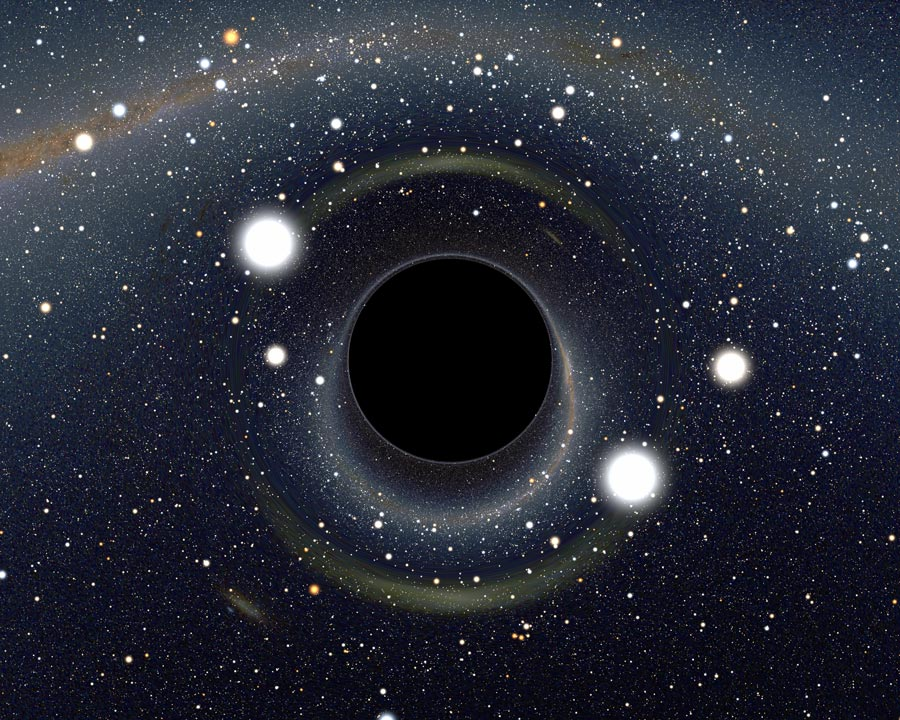
\includegraphics[width=.8\linewidth]{images/bhlens_riazuelo.jpg}
        \caption{NASA APOD 使用发光天体为单位进行追踪}
        \label{fig:nasa-apod}
    \end{subfigure}%
    \begin{subfigure}{.5\textwidth}
        \centering
        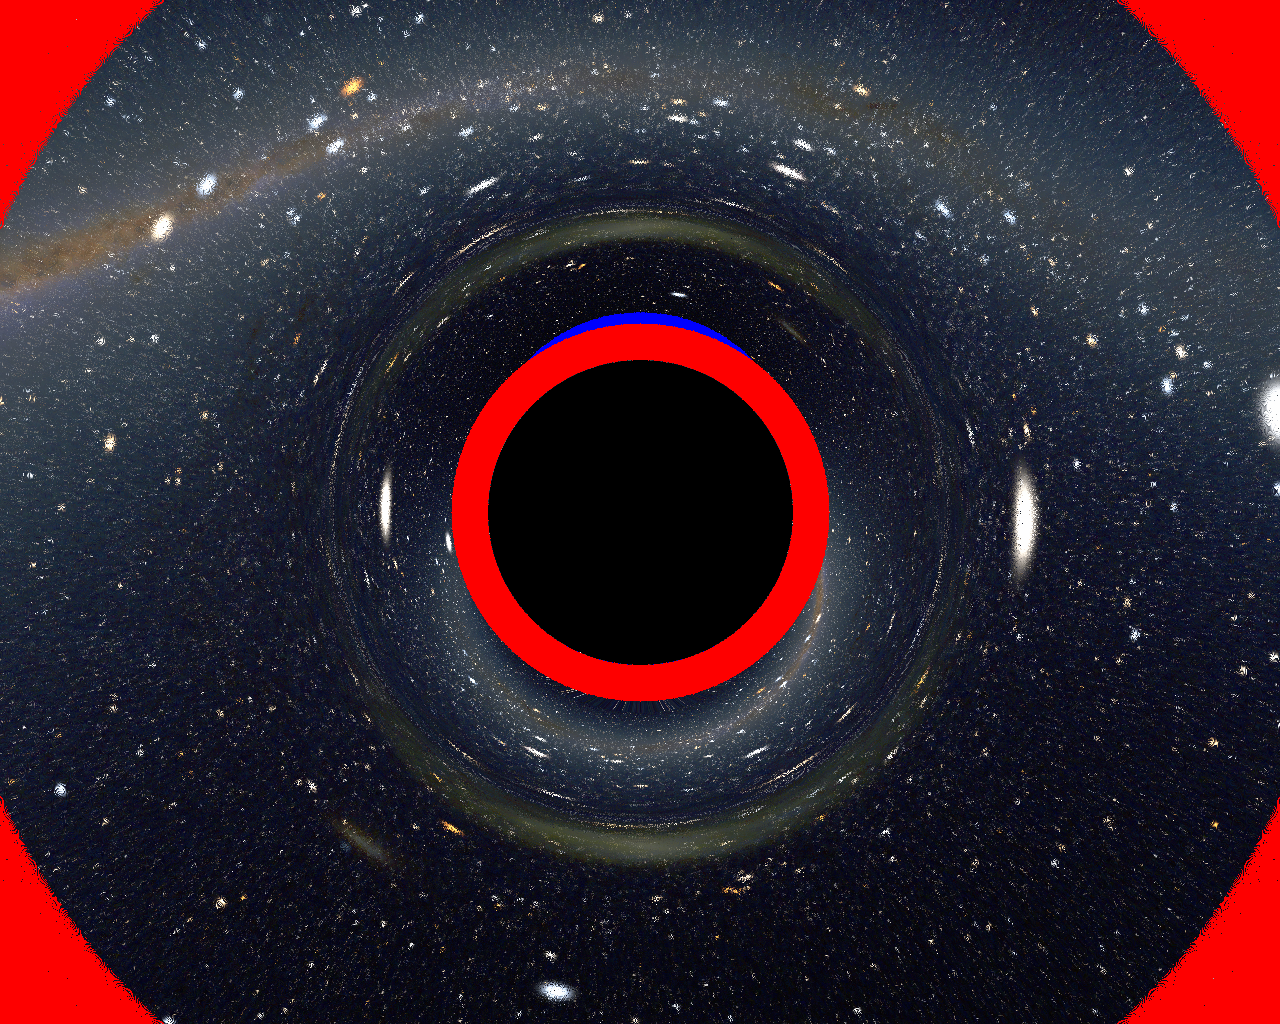
\includegraphics[width=.8\linewidth]{images/bhlens_erratum.png}
        \caption{使用像素为单位进行追踪}
        \label{fig:nasa-apod-erratum}
    \end{subfigure}
\end{figure}

图\ref{fig:nasa-apod}应该是有意为之\cite{riazuelo_seeing_2018},但不应该是人眼所看到的影像。

\paragraph{相机}
程序中拥有一个相机,相机有长宽比例、可视角度、世界坐标和观测角度等参数。以相机为中心,存在一个相机本地的坐标系,光子的发射角度由相机的参数,在相机本地坐标系下决定的。光线追踪需要一个本地坐标系到世界坐标系的转换。


\section{离线渲染}
传统的光线追踪程序是通过判断光线(直线)与平面是否相交来判断是否光线是否击中物体的。近年随着消费级硬件性能提升,实时渲染领域光线追踪有取代光栅化的趋势。但也只是刚刚起步,只有最顶级的消费级显卡才能以Full HD画质在大多数游戏中实现令人满意的光线追踪渲染效果(60 FPS)。

黑洞附近的光线路径不再是直线,不能使用简单的直线求交方式判断光线的hit和miss。每一束光线都要多次迭代才能获得光束的起点。实时渲染并非不可行,却是以精度为代价的。我想专注于离线渲染达到较好的效果。
\subsection{开发环境}
先在Mathematica上做数值模拟,再使用Python做可视化原型,Julia可能是更好的选择,因为Python实在是太慢了。

最后实现高精度的可视化模拟,可以选择C++和Rust。C++相对于Rust更容易整合GPU编程,实现星际穿越特效的物理引擎就是使用C++写的\cite{james_gravitational_2015}。
\paragraph{GPU与CPU模拟的优劣}
理论上来说,基于像素的并行计算应该是非常适合使用GPU进行模拟计算的。就像流体模拟和N体引力问题,大量的物体相互作用与大量的光子受引力影响而偏转。

但是有几点不同,
\begin{enumerate}
    \item 流体模拟不需要特别高的精度,逐步迭代光线追踪需要较高的积分精度,经过多次迭代累计误差会变得很大。
    \item 流体模拟不需要迭代运算,GPU主频普遍是CPU主频的$\nicefrac{1}{3}$左右,迭代速度会慢很多。
\end{enumerate}
对于本世代GPGPU,例如图灵架构,float64的运算速度只有float32的$\nicefrac{1}{32}$\cite{nvidia-turing-architecture-whitepaper}。我还是选择使用C++作为主要渲染实现方法,并尝试Vulkan Compute Shader在GPU上运算。

\subsection{程序输入}
程序不需要输入黑洞的质量,因为一切单位都是与黑洞质量成正比的。
\paragraph{吸积盘的几何与纹理}
吸积盘是一个圆环,需要设定吸积盘的内径与外径。还需要输入吸积盘的纹理,可以使用一维纹理也可以使用二维纹理。

\paragraph{天空盒纹理}
天空盒是六张分别代表上、下、左、右、前、后的正方形纹理,也可以是使用六面图层的一张图片,还可以使用六张拼接成一张的天空盒立方展开图。

\paragraph{相机设定}
唯一需要输入的坐标是相机的世界坐标,还需要相机本地坐标系中三个轴其中的两个在世界坐标系中的方向向量,知道其中两个可以计算第三个,用于确定相机的方向。相机x轴与y轴分别有一个视场(FoV)设定,用于确定光子发射角的最大值。

\subsection{光线追踪}
跟其他传统的光线追踪方法一样,光线是逆向追踪,从相机的坐标出发,这能极大的减轻运算量,但会导致采样的图片有噪点或者信息缺失,这个会通过多重采样来缓解。

三维坐标系跟二维坐标系下的光线追踪方法是类似的。根据史瓦西时空的对称性,我们需要确定一个光线偏转轴,然后根据这个偏转轴确定光子在测地线积分路径上的坐标。

\paragraph{光线偏转轴}
实现向量的旋转可以选择在极坐标系也可以选择在笛卡尔角坐标系下进行。我选择在笛卡尔坐标系下进行向量旋转。这样可以利用已知的欧拉角旋转矩阵简单的对向量进行旋转。光子的偏转轴确定为光子发射时的速度向量与相机位置向量的叉乘。

\paragraph{没有吸积盘的情况}
在黑洞没有吸积盘的情况下,只需要根据之前的推出的结论以光线的初始条件撞击参数b,确定光线是否会坠入黑洞。如果光线坠入黑洞,像素点的采样就是黑色的。如果光线没有坠入黑洞,则需要选定一个光线的积分终点,近似为光线传播到无限远处时的积分终点。如果直接求无限积分,就需要一套复杂的数值计算系统,其实是没有必要的。因为根据上面的结论,光线在距离黑洞20M以上之后就基本上不会受到空间弯曲的影响了。

我把近似无限远处的积分终点$r_1$设为2000M,这个范围完全足够了。整个测地线积分分为两段,从相机原点$r_0$到光线近点$r_3$,再从光线近点$r_3$到设定的积分终点$r_1$。其中有一段重复的积分范围,从$r_0$到$r_3$再从$r_3$到$r_0$,这两段互为相反数,实际积分的时候可以省掉重复的一段。

对测地线积分的结果为光线在一个极坐标平面上极角的变化量。也就是在三维坐标系中,光子对于偏转轴所要偏转的角度。我可以使用旋转矩阵\cite{rotation_matrix}绕轴$\vec{u}=\left(u_x,u_y,u_z\right)$旋转$\theta$度
\begin{equation}
    \begin{bmatrix}\cos\theta+u_{x}^{2}\left(1-\cos\theta\right) & u_{x}u_{y}\left(1-\cos\theta\right)-u_{z}\sin\theta & u_{x}u_{z}\left(1-\cos\theta\right)+u_{y}\sin\theta\\
        u_{y}u_{z}\left(1-\cos\theta\right)+u_{z}\sin\theta & \cos\theta+u_{y}^{2}\left(1-\cos\theta\right) & u_{y}u_{z}\left(1-\cos\theta\right)-u_{x}\sin\theta\\
        u_{z}u_{x}\left(1-\cos\theta\right)-u_{y}\sin\theta & u_{z}u_{y}\left(1-\cos\theta\right)+u_{x}\sin\theta & \cos\theta+u_{z}^{2}\left(1-\cos\theta\right)
        \end{bmatrix}
\end{equation}

旋转完后就能得到光子在$r_1$的位置向量,实际上近似于光子在$r_1$的速度向量,也是最终在天空盒上采样的方向向量。

\paragraph{有吸积盘的情况}
黑洞如果拥有吸积盘,上面两种情况的光线都有可能与吸积盘相交。

首先可以通过计算光子轨道近点排除完全不可能与吸积盘相交的光子,也就是光子不会进入由吸积盘圆环内圆与外圆所在的同心球壳之间的空间,光子会直接射向无限远处的天空盒。

如果光线进入吸积盘同心球壳,存在三种情况,

\begin{itemize}
    \item 光子近点在吸积盘范围内,需要从外径积分到近点再积分到外径
    \item 光子近点在吸积盘内径以内,最终坠入黑洞,
    \item 光子近点在吸积盘内径以内,则从吸积盘外径积分到内径
\end{itemize}

判断吸积盘与光子相交,通过判断光子在吸积盘范围\footnote{\label{accretion_disk_area}吸积盘外径所在球壳与内径所在球壳之间的空间}内是否穿过赤道面。有两个充分条件(sufficient condition)可以判断,
\begin{enumerate}
    \item 光子在吸积盘范围内的运动极角变化大于$\ang{180}$,因为光子绕中心天体运动,极角变化超过$\ang{180}$必定与赤道面相交;
    \item 光子在吸积盘范围内运动的起始坐标与终止坐标的y轴部分符号不同
\end{enumerate}

当其中一条满足就要进入光线与吸积盘相交的采样过程,这个过程是整个渲染中最消耗CPU时间的部分。

可以选择数值求解的方法得到光子进入吸积盘范围后达到吸积盘所需要的偏转角度,也可以通过逐步模拟的方法对光线进行追踪,我选择后者。为了提高速度,我选择了可变步长的逐步追踪,当光子越接近赤道面时,步长越小,这样能有效减少迭代次数。最终光线与吸积盘相交时的坐标就可以转换为吸积盘纹理的采样坐标。

\subsection{采样与抗锯齿}
\paragraph{纹理采样}程序中需要用到纹理采样的地方有两个,天空盒与吸积盘。天空盒的采样只需要一个光线的速度向量,在六面天空盒上对应采集纹素。吸积盘的纹理横轴均匀分布在吸积盘的一周,纵轴则是从外径到内径。吸积盘的采样需要光子打在吸积盘上的绝对坐标(赤道面上的二维坐标),转换为极坐标后就是纹素的二维坐标。

\paragraph{抗锯齿}
程序的抗锯齿是一个简单的MSAA (Multisample Anti-Aliasing)抗锯齿,这个过程发生在光子从相机出发的时候,而不是对天空盒和吸积盘采样的时候,因为黑洞本身也需要抗锯齿,不只是纹理。

抗锯齿的采样点选取是一个简单的均匀分布随机采样,给光子的发射时的速度向量增加一个与分辨率成反比的摄动(perturbation)。将多个光线追踪后的采样值叠加得到最后的单个像素颜色。

\subsection{后处理}
程序有一个图像后处理功能,是给吸积盘加上bloom的效果。为了做到这个,需要一个光源缓冲区记录吸积盘本身,因为只有吸积盘是发光的。将光源缓冲区进行高斯模糊,得到吸积盘的bloom效果。将光源缓冲区与原始的颜色缓冲区叠加后得到一张HDR图片,对HDR图片进行Tone Map和伽马矫正后得到最终的显示图像。
\begin{figure}[H]
    \centering
    \begin{subfigure}{.5\textwidth}
        \centering
        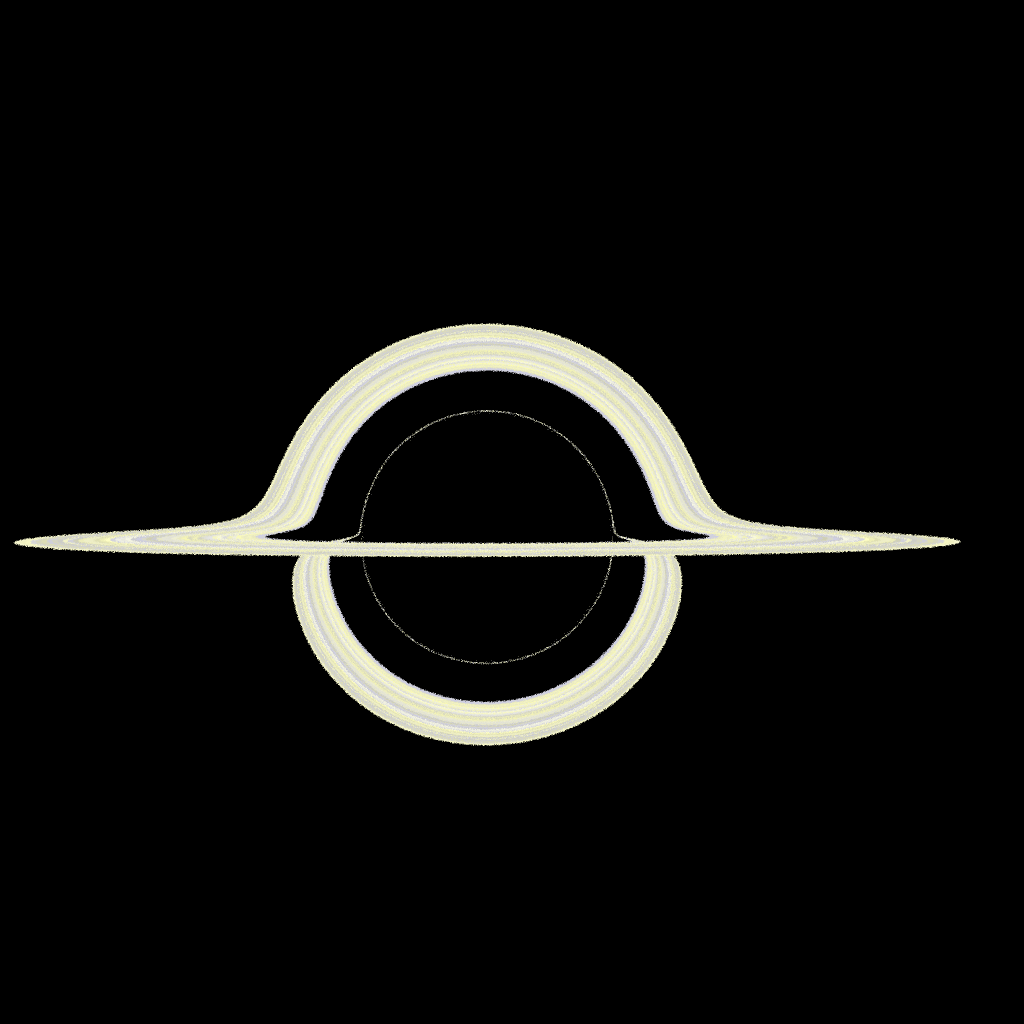
\includegraphics[width=.8\linewidth]{images/no-bloom.png}
        \caption{未处理图像}
        \label{fig:no-bloom}
    \end{subfigure}%
    \begin{subfigure}{.5\textwidth}
        \centering
        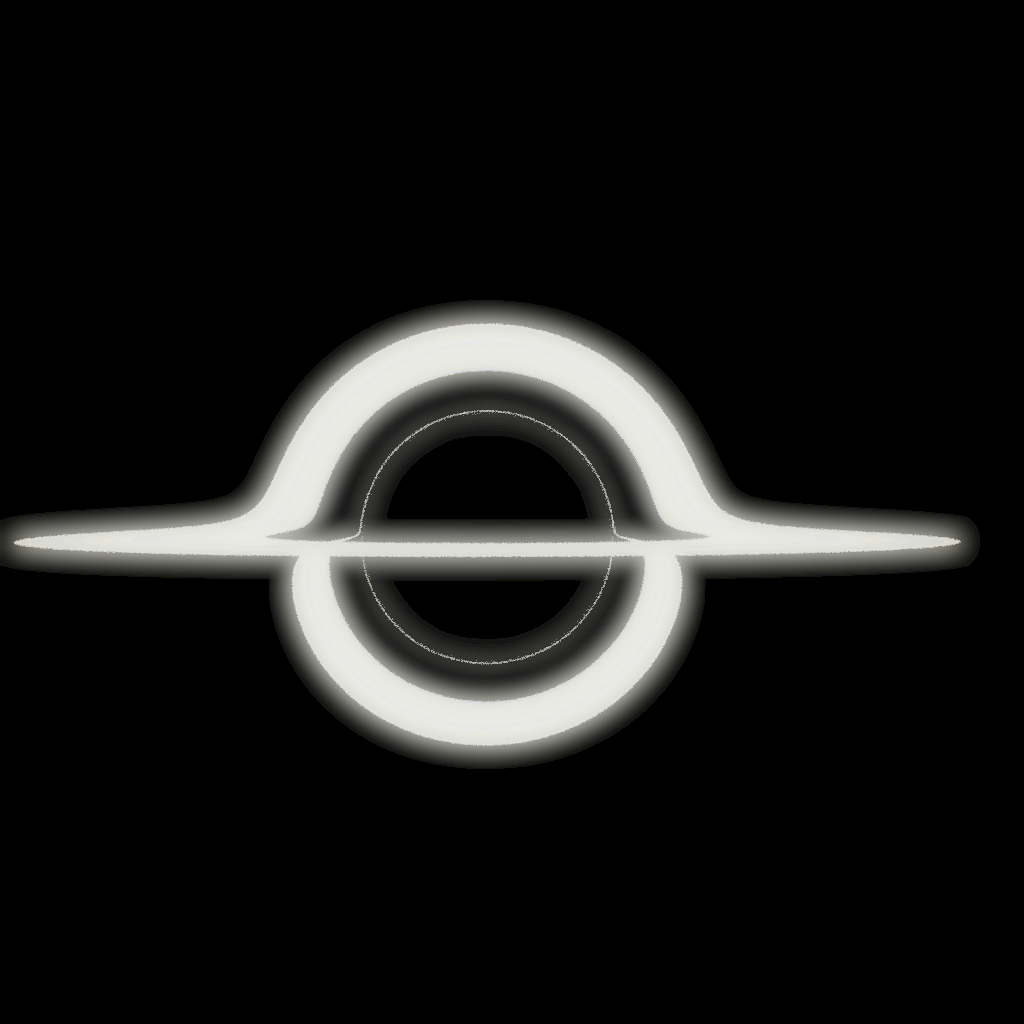
\includegraphics[width=.8\linewidth]{images/bloom.png}
        \caption{blooming后的图像}
        \label{fig:bloomed}
    \end{subfigure}
\end{figure}


\subsection{成像}
这里使用一个棋盘背景作为天空盒来演示光线偏折的效果,
\begin{figure}[H]
    \centering
    \begin{subfigure}{.5\textwidth}
        \centering
        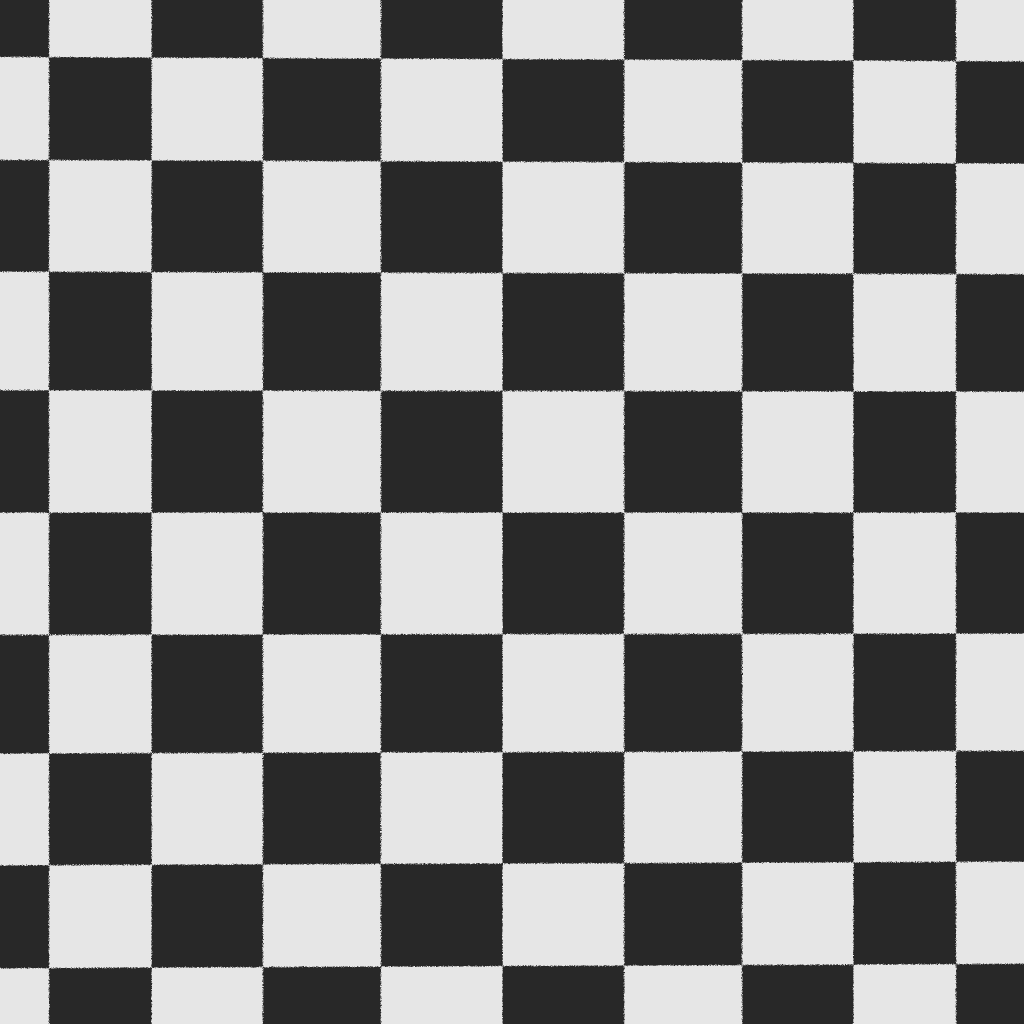
\includegraphics[scale=0.2]{images/chessboard.png}
        \caption{棋盘天空盒,没有黑洞的时候看到的背景}
        \label{fig:chessboard} % label 用来在文中索引
    \end{subfigure}%
    \begin{subfigure}{.5\textwidth}
        \centering
        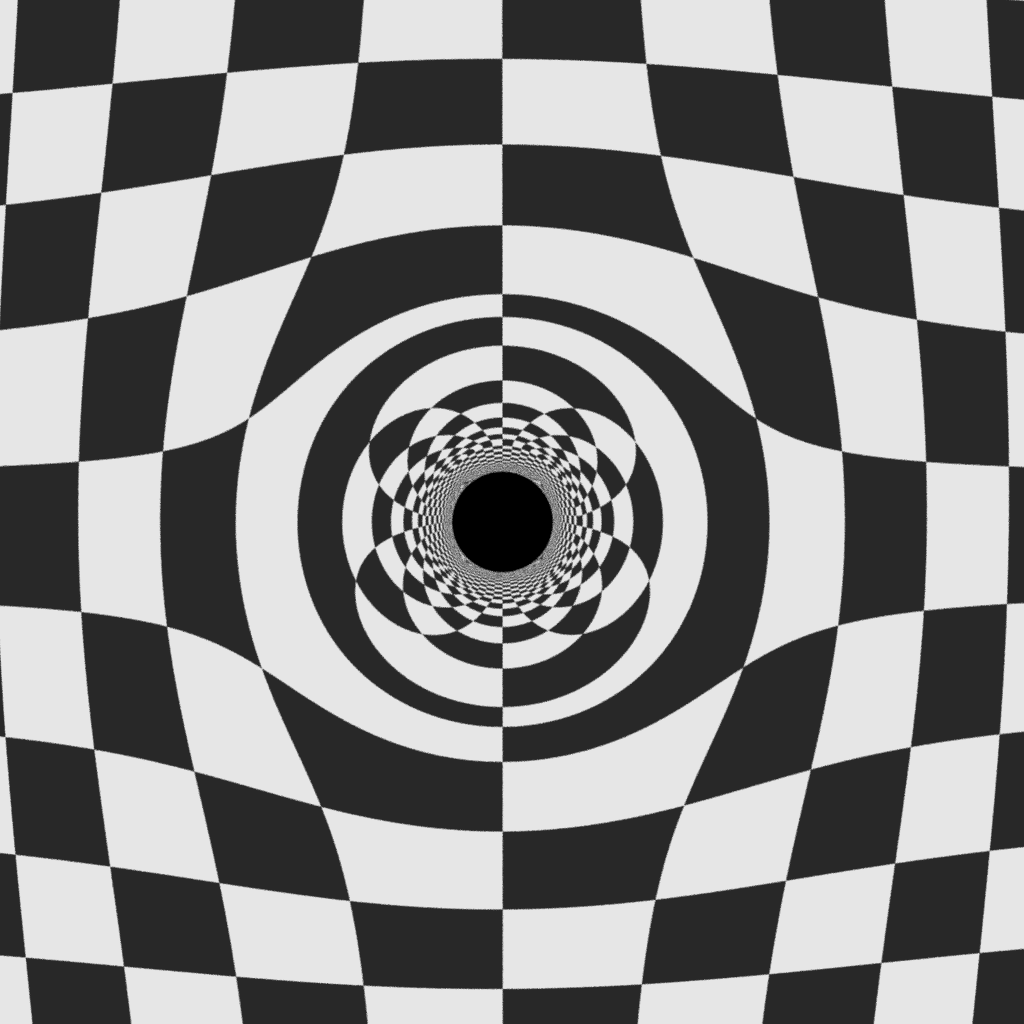
\includegraphics[scale=0.2]{images/blackhole_chessboard.png}
        \caption{距离黑洞100M}
        \label{fig:blackhole-chessboard} % label 用来在文中索引
    \end{subfigure}
\end{figure}

光线越接近黑洞,产生的偏折越大,当光线靠近光子轨道$r=3M$处时,光子会开始短暂环绕黑洞\ref{fig:camera_view_orbit},光线会来自天空盒的各个面,所以黑洞附近的图像方格非常密集。

使用一个\ang{360}全景图作为天空盒可以从另一个角度直观感受光线的偏折,
\begin{figure}[H]
    \centering
    \begin{subfigure}{.5\textwidth}
        \centering
        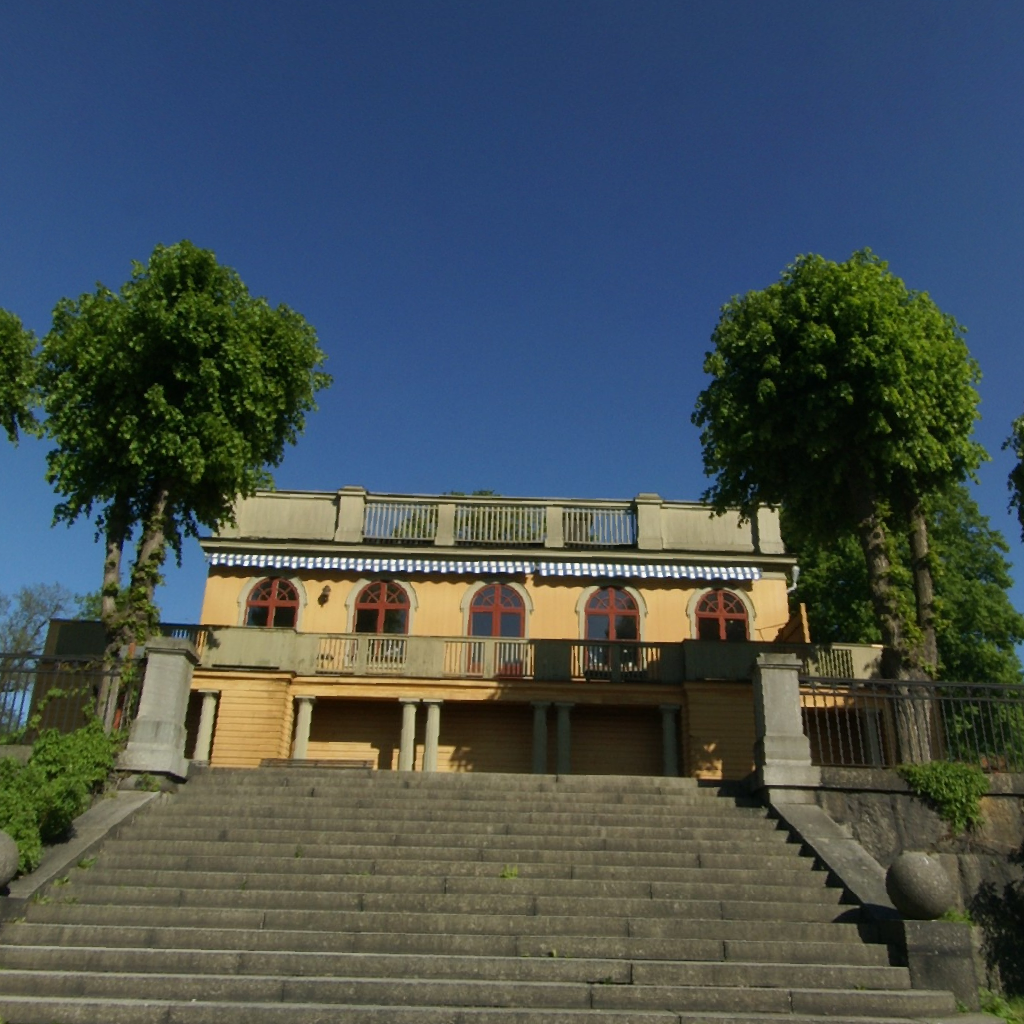
\includegraphics[width=.8\linewidth]{images/building.png}
        \caption{天空盒的一面}
        \label{fig:building}
    \end{subfigure}%
    \begin{subfigure}{.5\textwidth}
        \centering
        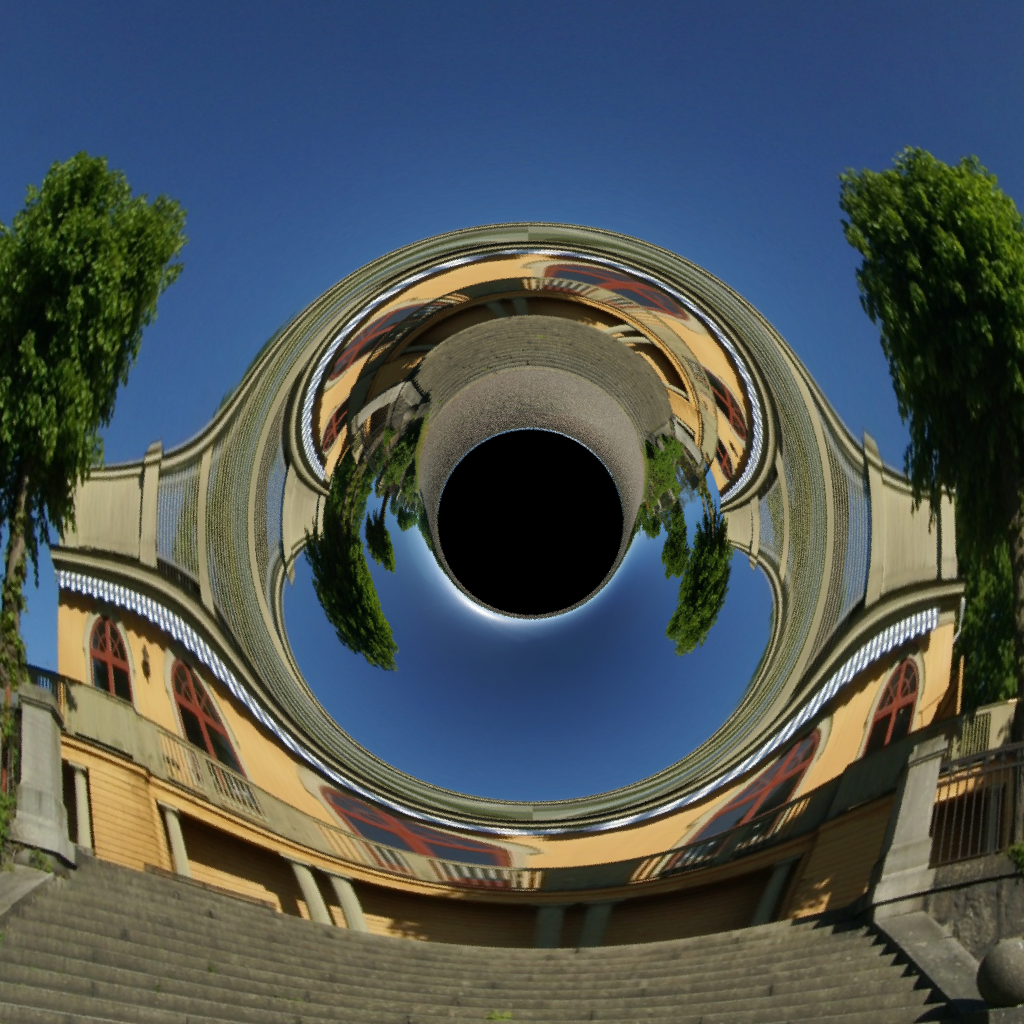
\includegraphics[width=.8\linewidth]{images/building_distort.png}
        \caption{变形后的图像}
        \label{fig:building_distort}
    \end{subfigure}
\end{figure}
从这个发生形变的图像可以看出一些黑洞附近光线轨迹的特点,
\begin{enumerate}
    \item 两旁的树有可见的像有两个,一个时数的主像,在图像的两侧,在接近黑洞中心的位置有一个倒立的次级像。这很像凸透镜的效果。
    \item 房子二楼的栅格围栏刚好在黑洞的后面,整个围栏的产生巨大的形变,但围栏是完整的,信息并没有丢失。
    \item 围栏形成了一个环状结构,其实是最外层的爱因斯坦环
    \item 接近黑洞视界下面的部分有一束白光,这束白光是变形后被拉长的太阳,在天空盒的背面,这是黑洞引力透镜成像与凸透镜不一样的地方。
\end{enumerate}
如果将图\ref{sub@fig:building_distort}放大,在靠近黑洞视界的地方可以清楚的看到后方的太阳。这是太阳的次级像(二次像)\footnote{主像(一次像)在哪?太阳的主像并没有在图片中展示出来,但并不等于没有。太阳的主像来自摄像机的背后,只要摄像机的视场够大就能看到主像。}

\begin{figure}[H]
    \centering
    \begin{subfigure}{.33\textwidth}
        \centering
        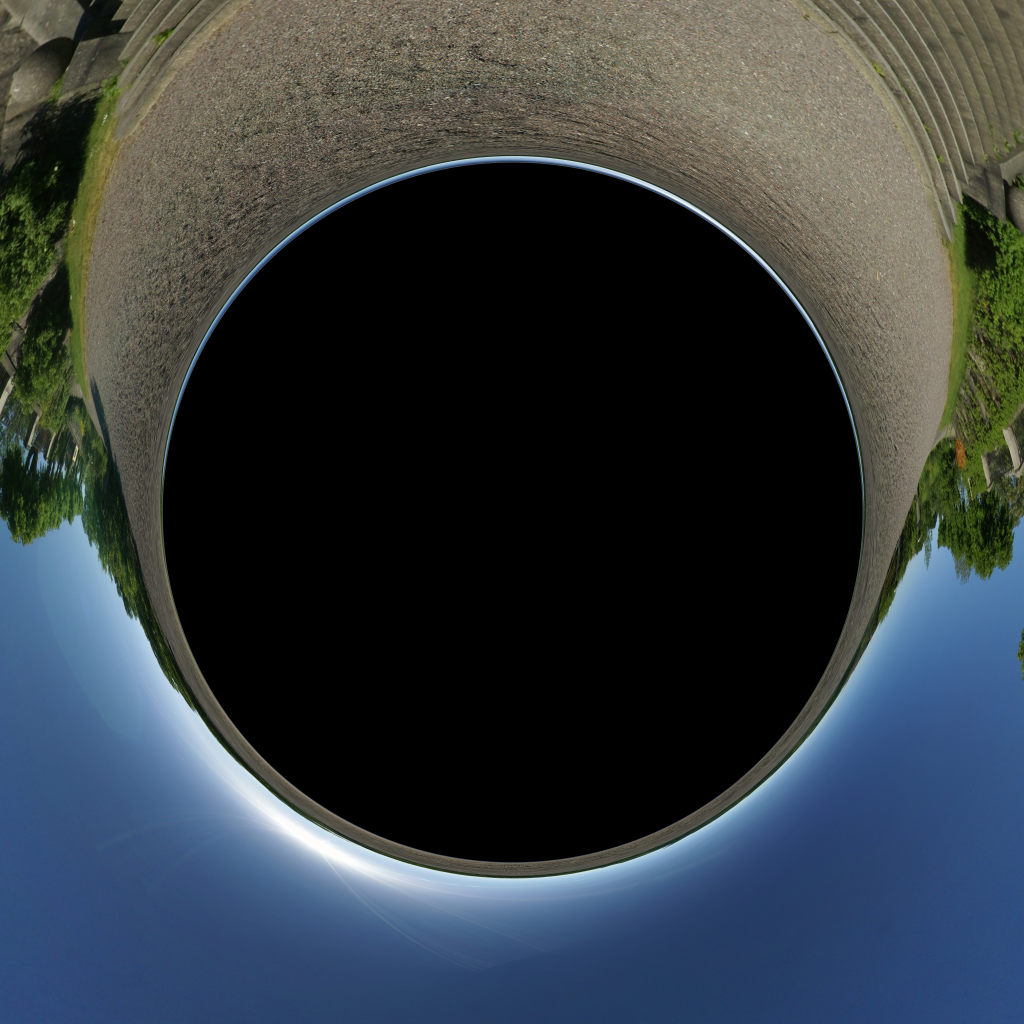
\includegraphics[width=.95\linewidth]{images/zoomin_6x.png}
        \caption{放大6倍}
        \label{fig:zoomin-6x} % label 用来在文中索引
    \end{subfigure}%
    \begin{subfigure}{.33\textwidth}
        \centering
        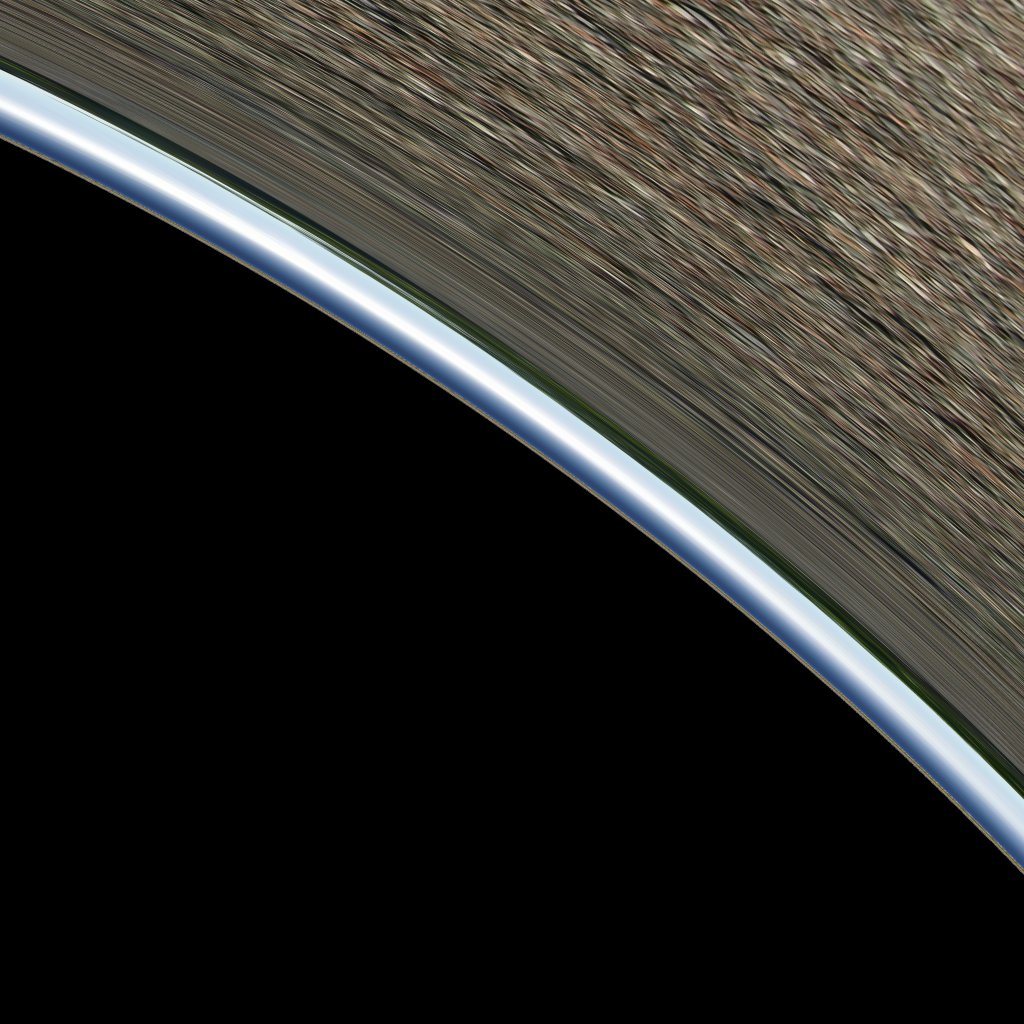
\includegraphics[width=.95\linewidth]{images/zoomin_60x.png}
        \caption{放大60倍}
        \label{fig:zoomin-60x} % label 用来在文中索引
    \end{subfigure}
    \begin{subfigure}{.33\textwidth}
        \centering
        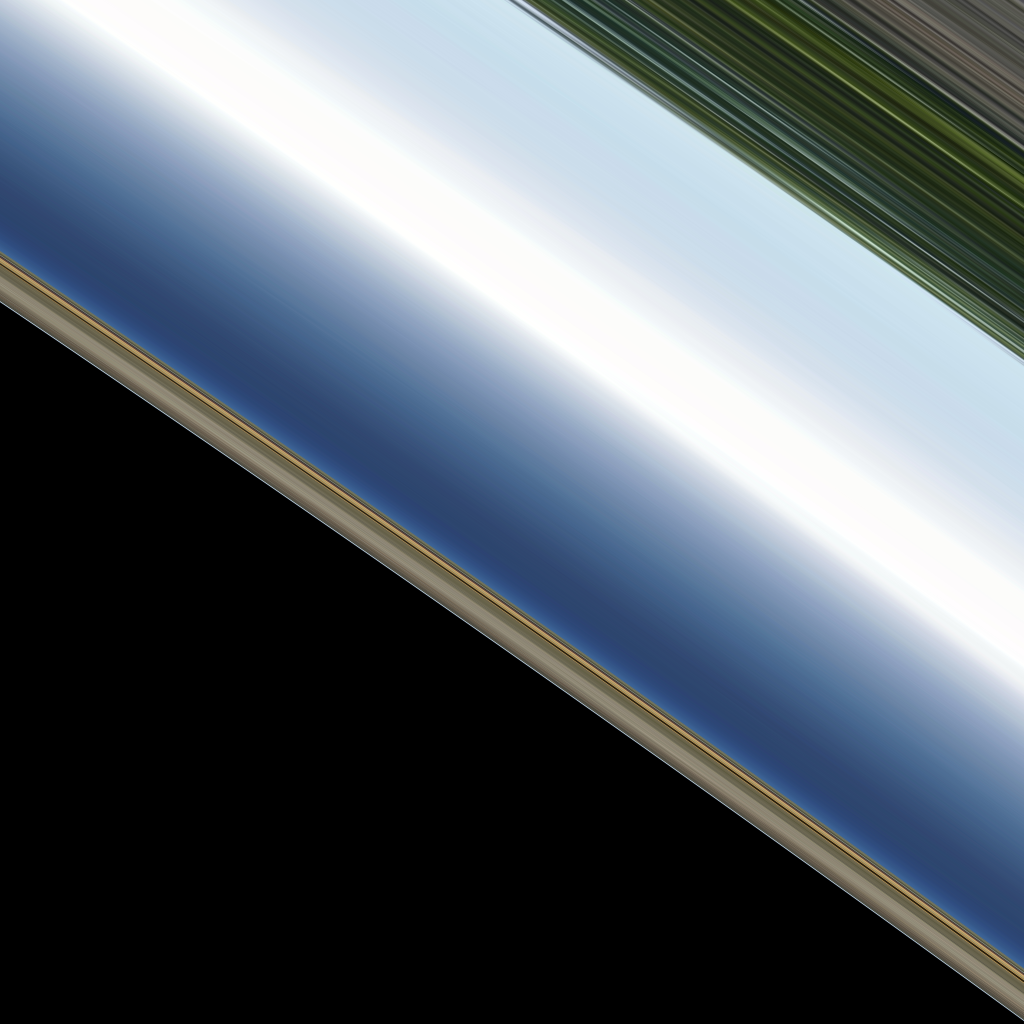
\includegraphics[width=.95\linewidth]{images/zoomin_600x.png}
        \caption{放大600倍}
        \label{fig:zoomin-600x}
    \end{subfigure}%
\end{figure}


如果再放大\ref{fig:zoomin-6x}的右上角的视界部分得到\ref{fig:zoomin-60x},可以看到后方太阳的三次像,这是第二个爱因斯坦环。

\begin{figure}[H]
    \centering
    \begin{subfigure}{.45\textwidth}
        \centering
        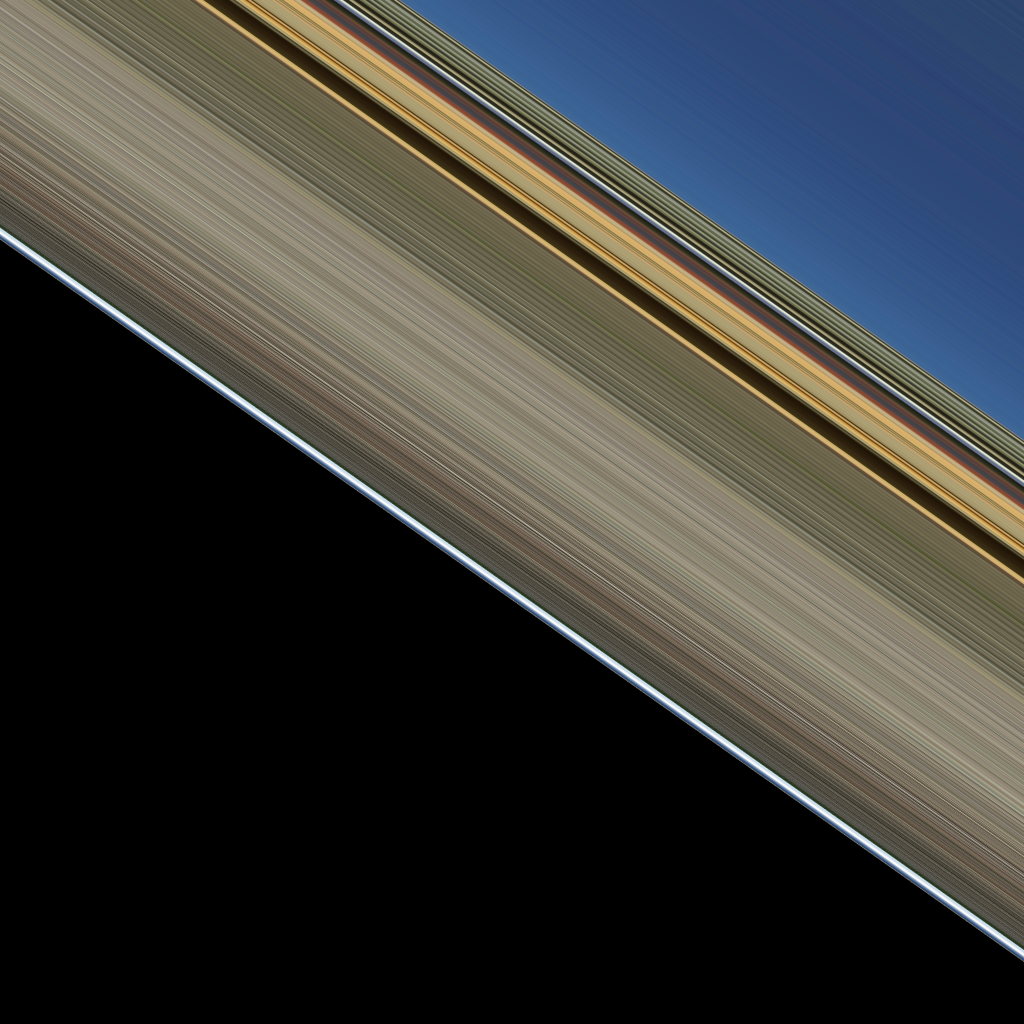
\includegraphics[width=.8\linewidth]{images/zoomin_6000x.png}
        \caption{放大6000倍}
        \label{fig:zoomin-6000x}
    \end{subfigure}
    \begin{subfigure}{.45\textwidth}
        \centering
        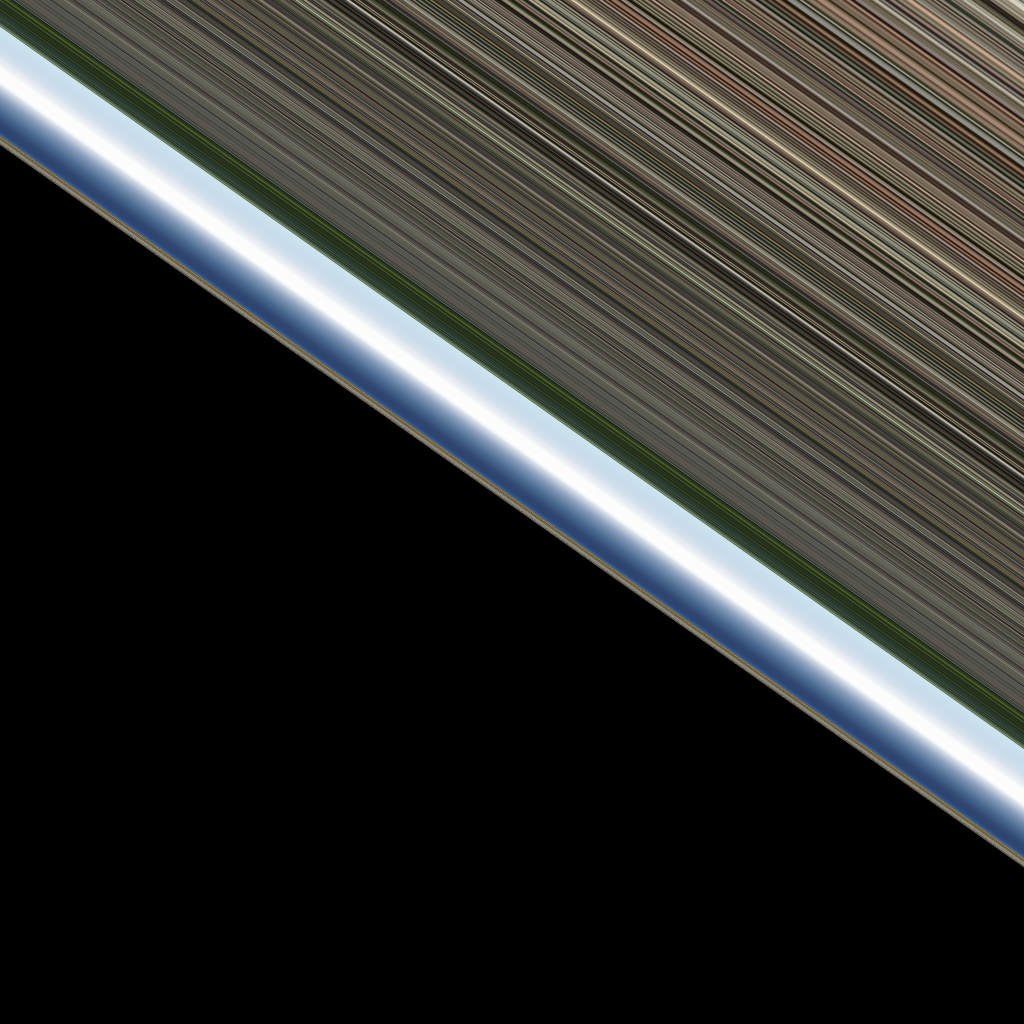
\includegraphics[width=.8\linewidth]{images/zoomin_60000x.png}
        \caption{放大60000倍}
        \label{fig:zoomin-60000x}
    \end{subfigure}
\end{figure}

将\ref{fig:building_distort}放大60000倍,这是太阳的四次像,第三个爱因斯坦环。四次像说明这束光线环绕黑洞转了两圈半。注意到图\ref{fig:zoomin-60x}与图\ref{fig:zoomin-60000x}是非常相似的两张图片,这意味着黑洞边界的图像是可以无限细分的。光线每围绕黑洞转一圈,就会在靠近黑洞视界的形成一个完整的世界的像。

\paragraph{爱因斯坦环}
爱因斯坦环是指星星的主像与次级像对称地成像在黑洞的两侧,两侧光线剧烈扭曲而形成的一个环状结构。爱因斯坦环太空中会比较明显,因为背景是黑色的,会显示为一个黑洞周围的亮环。
\begin{figure}[H]
    \centering
    \begin{subfigure}{.5\textwidth}
        \centering
        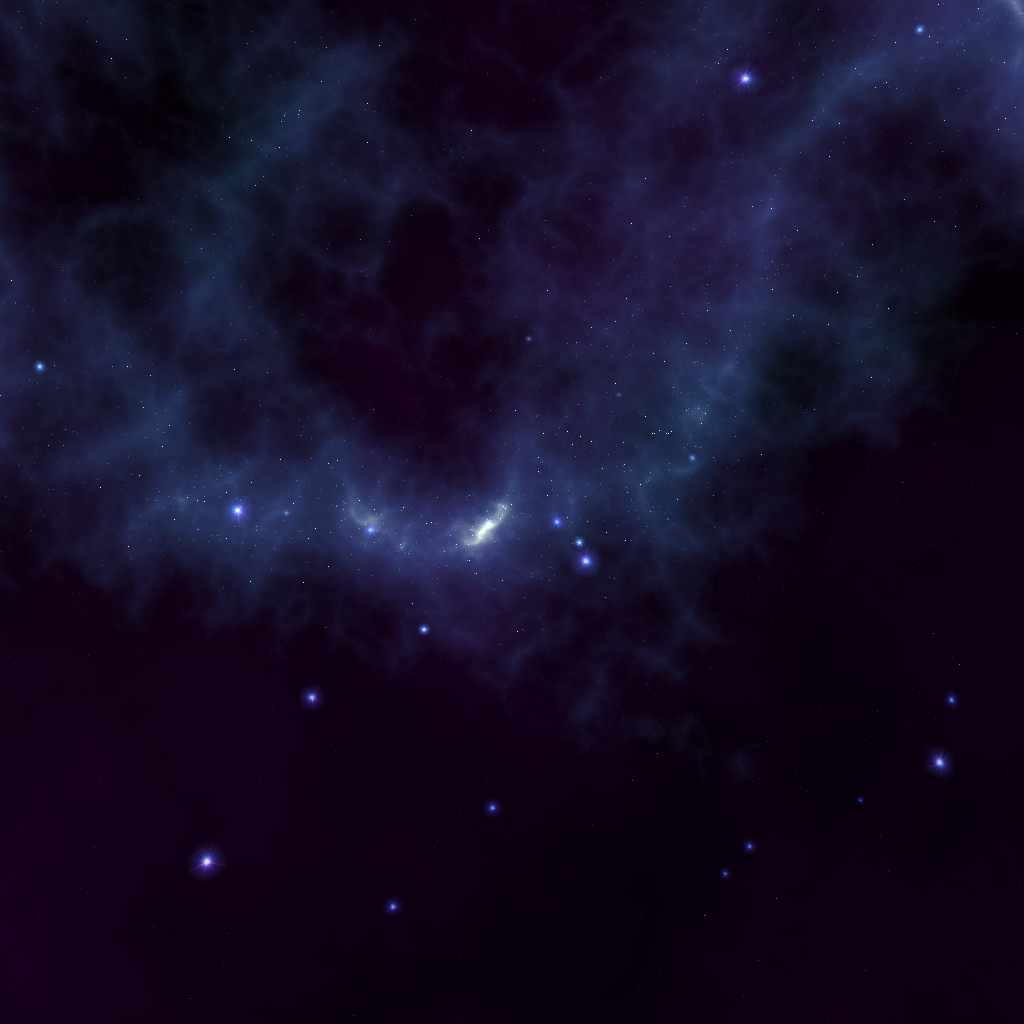
\includegraphics[width=.8\linewidth]{images/no_ring.png}
        \caption{背景星空}
        \label{fig:no-ring}
    \end{subfigure}%
    \begin{subfigure}{.5\textwidth}
        \centering
        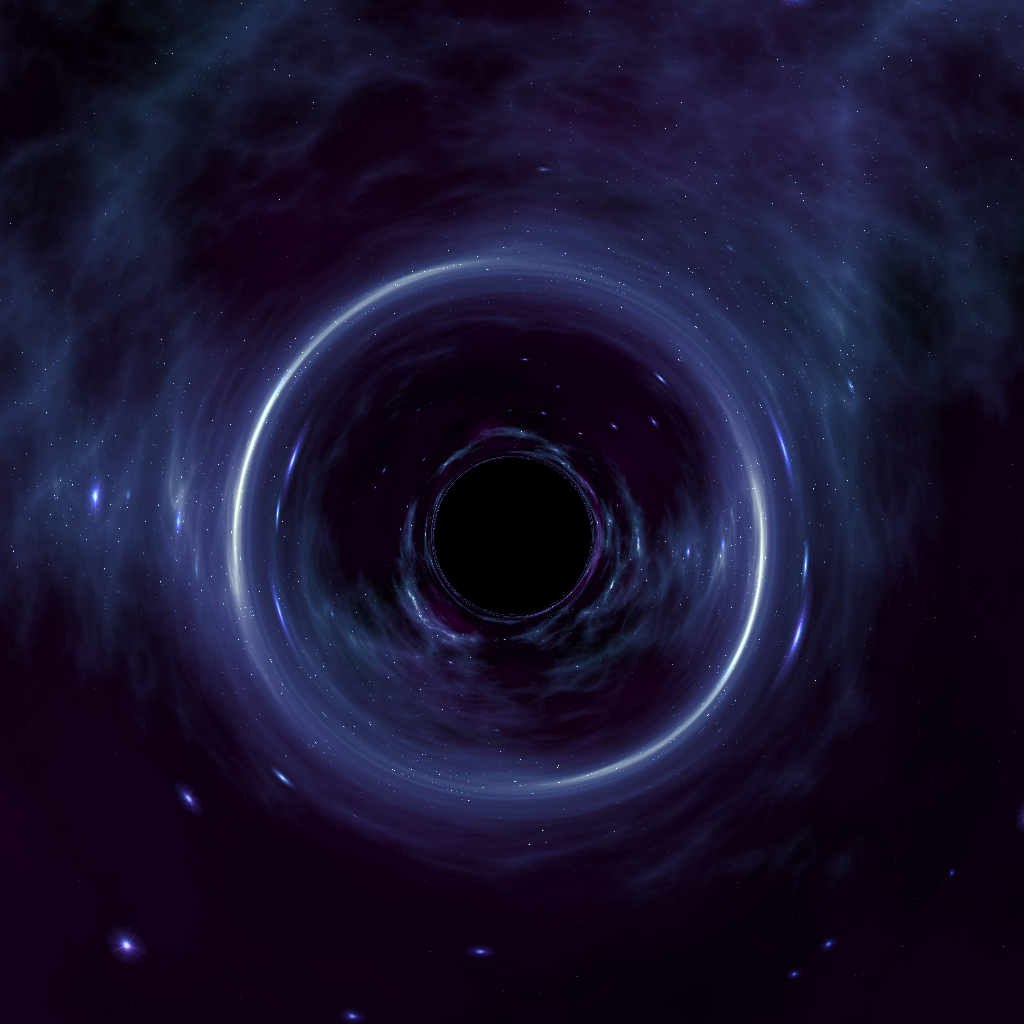
\includegraphics[width=.8\linewidth]{images/einstein_ring.png}
        \caption{距离黑洞64M}
        \label{fig:einstein-ring}
    \end{subfigure}
\end{figure}
图中中心的光线被分散到黑洞的四周,形成一个光环。

\subsubsection{吸积盘}
出于直观考虑,我制作了一个方格型的吸积盘贴图,吸积盘设定是一个无线薄的圆环,原则上从侧面看吸积盘是看不到的,将贴图的首尾相连形成一个环状就是吸积盘的外观。
\begin{figure}[H]
    \centering
    
\includegraphics[scale=0.5]{images/flag.png}
    \caption{吸积盘贴图}
    \label{fig:disk-flag-texutre} % label 用来在文中索引
\end{figure}
从正上方观察黑洞会看到吸积盘是一个正圆环,光线会被黑洞拉向中心(吸积盘观察到的内径与外径相比实际的内外径偏小),
\begin{figure}[H]
    \centering
    \begin{subfigure}{.5\textwidth}
        \centering
        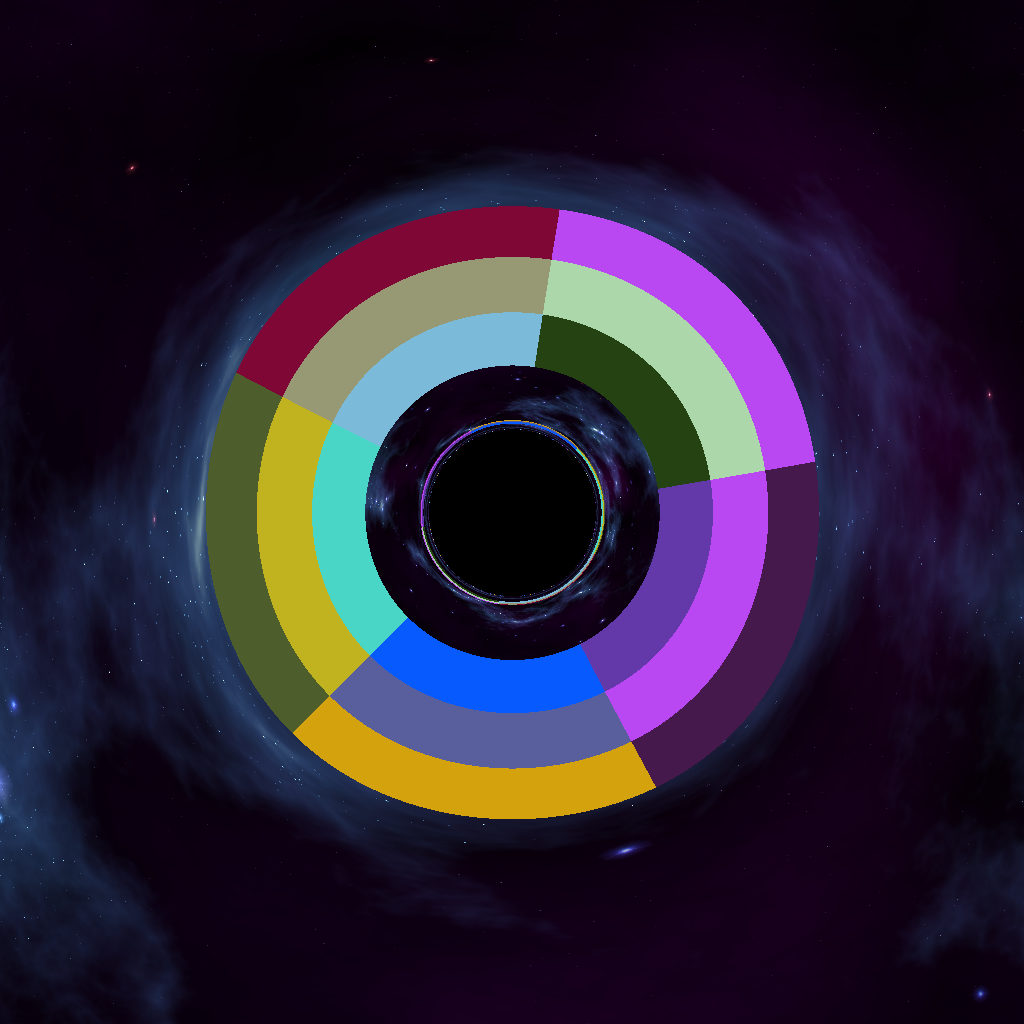
\includegraphics[width=.8\linewidth]{images/disk_top.png}
        \caption{上方观察黑洞与吸积盘}
        \label{fig:disk_top}
    \end{subfigure}%
    \begin{subfigure}{.5\textwidth}
        \centering
        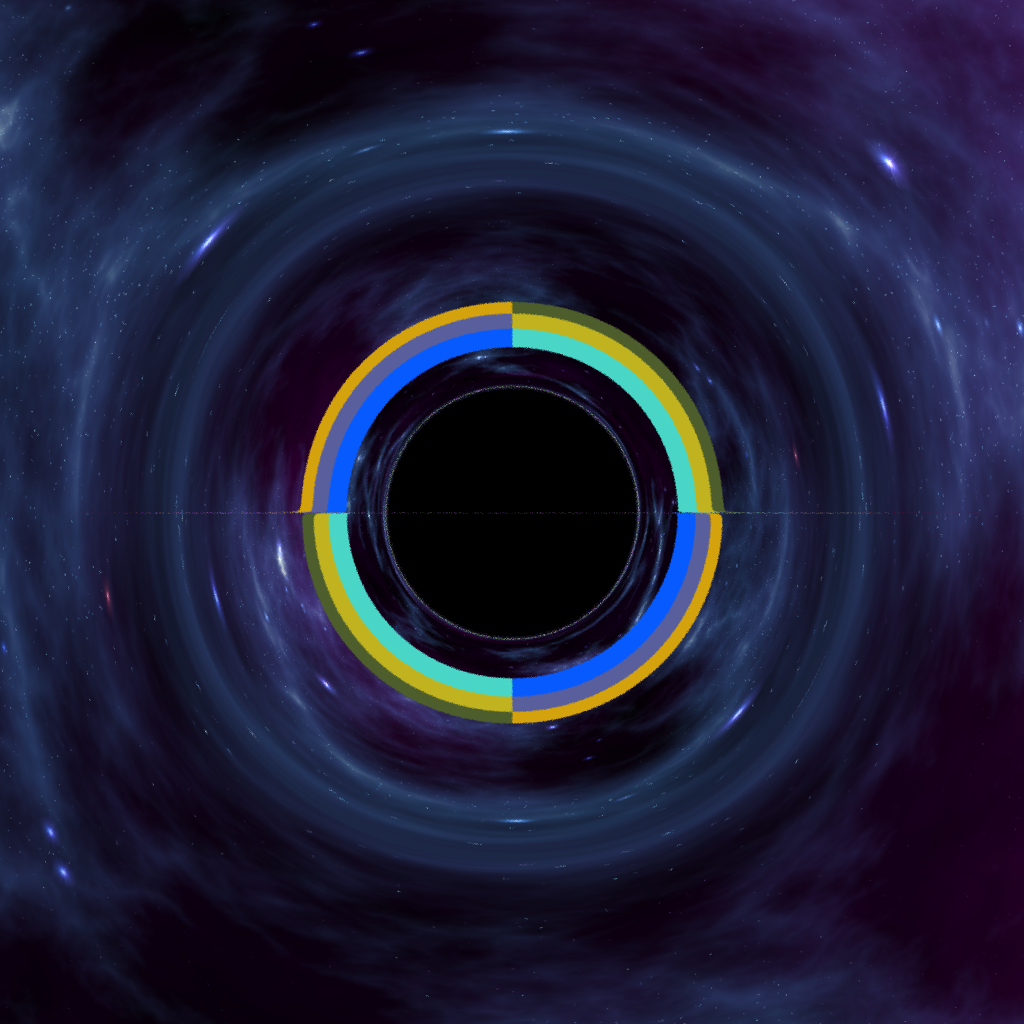
\includegraphics[width=.8\linewidth]{images/equatorial_plane.png}
        \caption{在赤道面观察}
        \label{fig:einstein-ring}
    \end{subfigure}
\end{figure}
在赤道面上观察,可以看到背面的吸积盘所成的两个对称像。

在赤道面上方一点点,可以观察到黑洞正面吸积盘的主像与背面的主像(上方半圆)衔接,而背面的次级像(下方半圆)与处在黑洞视界边缘的黑洞正面吸积盘的次级像衔接(下方半圆在赤道上迅速缩小到黑洞视界边缘)。
\begin{figure}[H]
    \centering
    \begin{subfigure}{.5\textwidth}
        \centering
        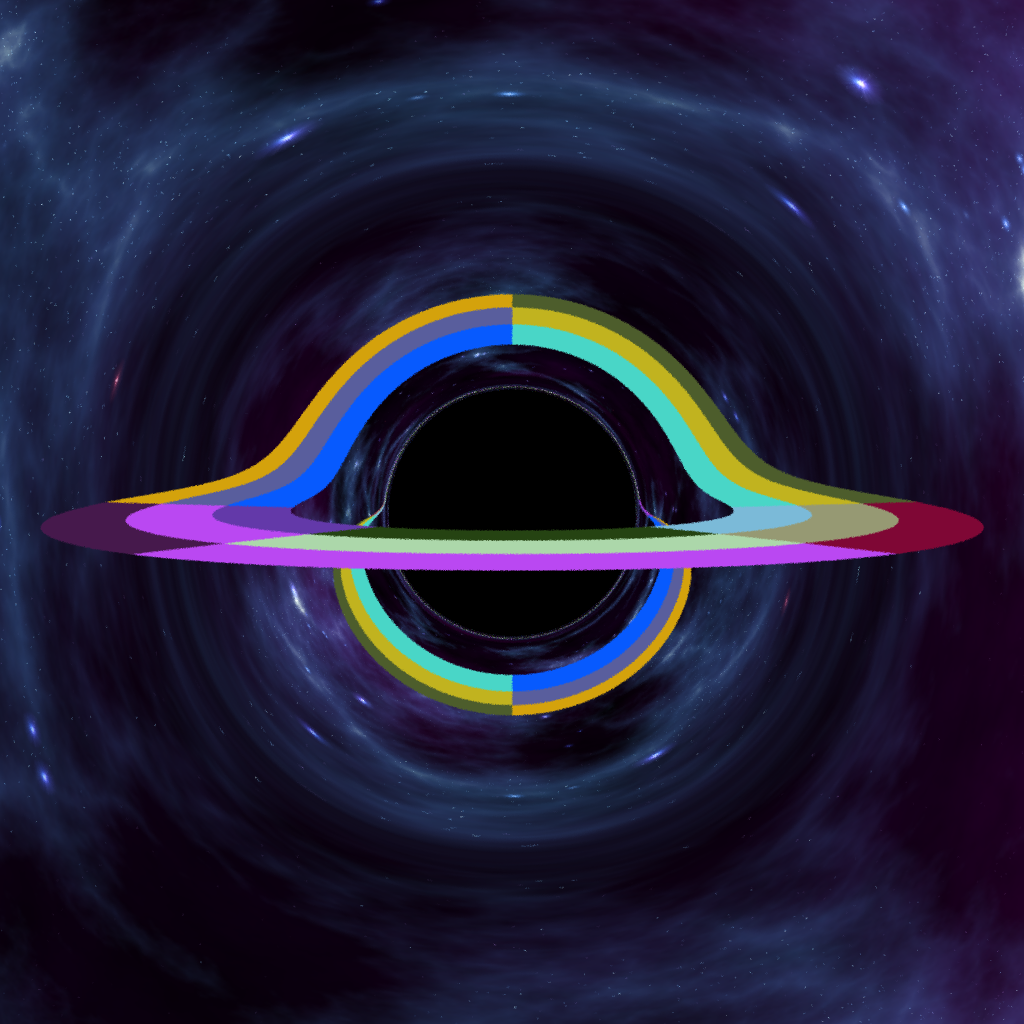
\includegraphics[width=.8\linewidth]{images/above_equatorial_plane.png}
        \caption{上方观察黑洞与吸积盘}
        \label{fig:above_equatorial_plane}
    \end{subfigure}%
    \begin{subfigure}{.5\textwidth}
        \centering
        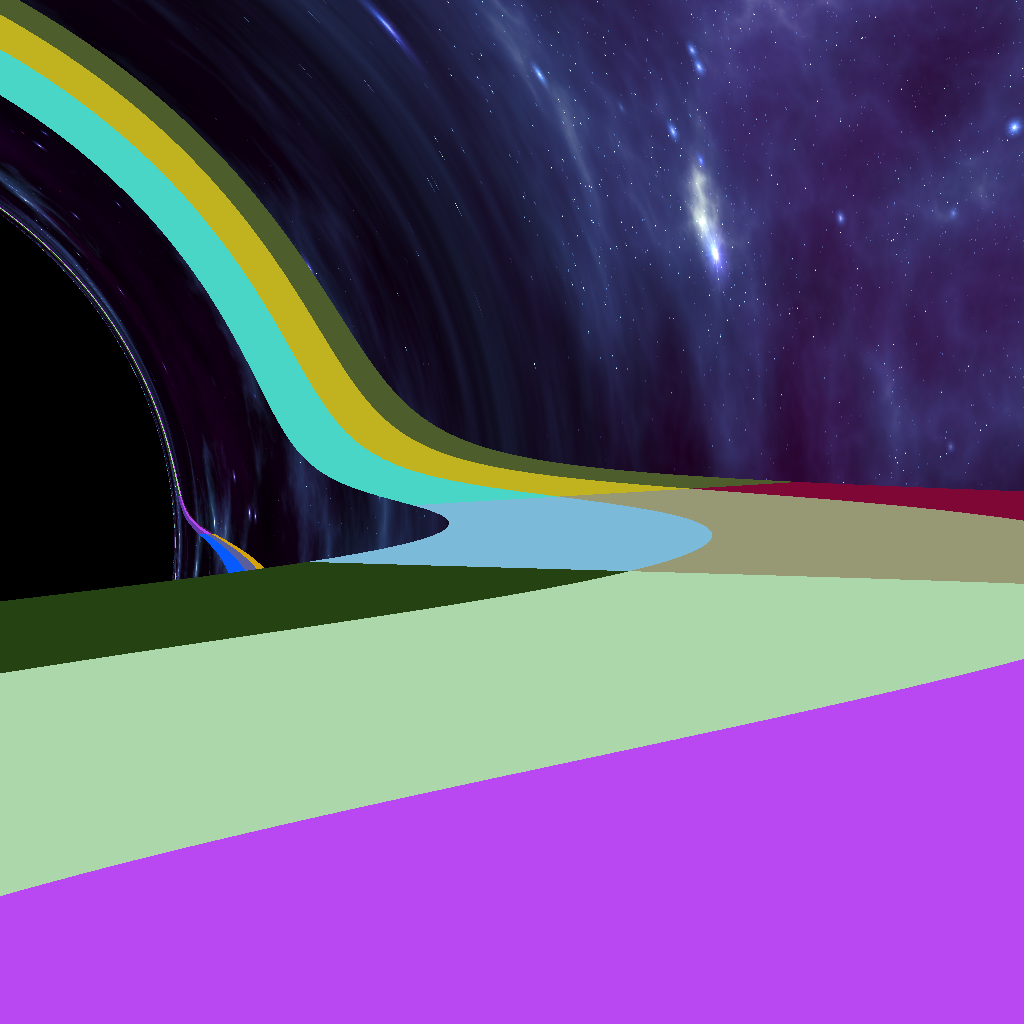
\includegraphics[width=.8\linewidth]{images/stand_on_disk.png}
        \caption{相机在吸积盘上观察}
        \label{fig:einstein-ring}
    \end{subfigure}
\end{figure}

\subsection{用户图形界面}
用QT框架给程序包裹了一层图形界面,方便使用。程序的前端图形界面与后端渲染引擎是分离的,引擎完全不依赖图形界面,使用命令行也可以实现其功能。
\begin{figure}[H]
    \centering
    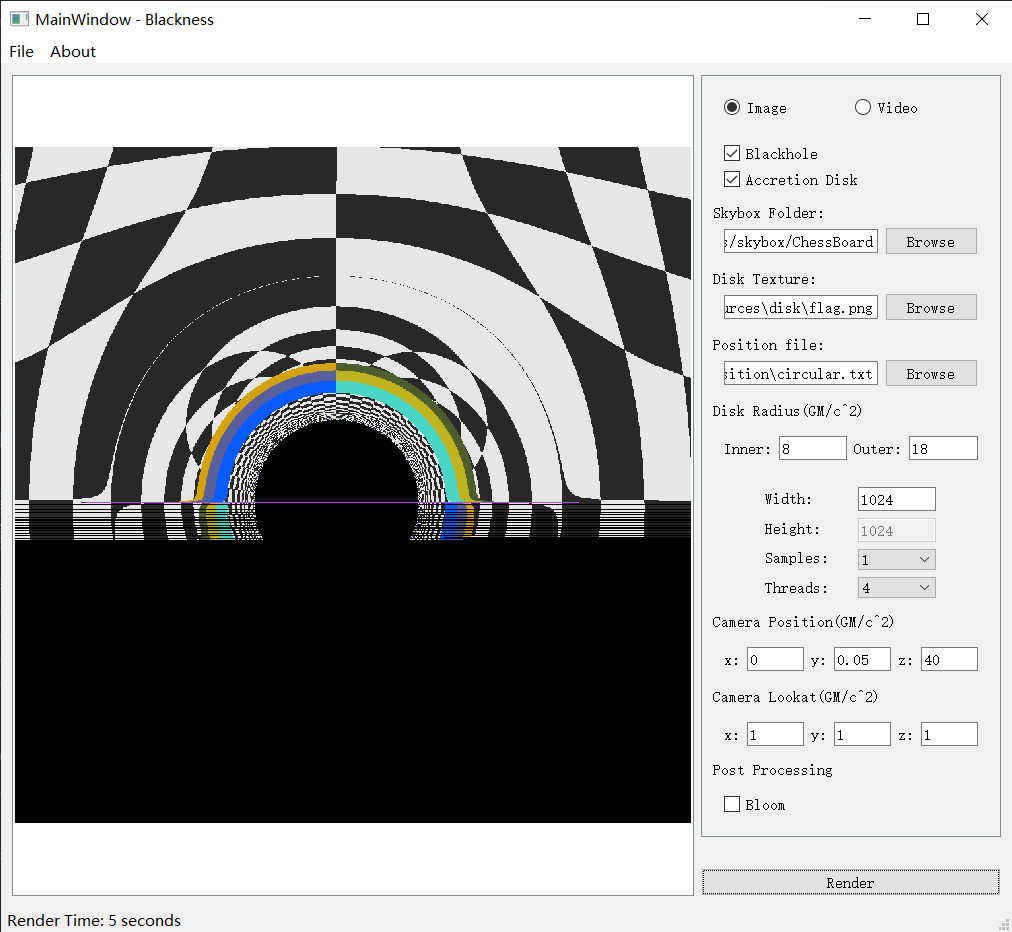
\includegraphics[scale=0.5]{images/gui.png}
    \caption{程序界面}
    \label{fig:gui} % label 用来在文中索引
\end{figure}
窗体的左侧是渲染状态,可是实时预览渲染的情况,这样就省去了进度条的显示。右侧是程序输入与设定,基本上涵盖了渲染所需要设定的参数与纹理。图片渲染完成后可以保存到硬盘上。

\subsection{动态模拟}
动态的模拟可以更直观的看到,运动的相机是如何感知黑洞周围的光线的,或者演示旋转的吸积盘是如何被黑洞引力拉扯的。

程序有一个生成视频的接口,使用的是ffmpeg的C++库。用户需要输入每一帧相机的坐标与方向数据到文件里,使用接口读入文件就可以生成视频文件了。视频编码需要的是每一帧的图像数据,我是用的是8比特3通道图像,每一帧的生成都可以在GUI中预览,每一帧渲染完成后,将图像使用VP9编码,最后一帧生成后,将编码后的视频放进MP4容器中存入硬盘。

\subsection{性能}
我尝试过使用GPU进行渲染,一般而言,GPU在并行计算上相对于CPU有非常大的优势,特别是这种以像素为单位的渲染。但是在这种高精度渲染的目的下,GPU并不能胜任,有几点原因,
\begin{enumerate}
    \item GPU主频不高,迭代循环光线追踪是比较慢的
    \item 高精度迭代追踪需要双精度浮点,甚至128位浮点数。本世代GPU只有非常小的核心面积是用于双精度浮点数计算的,速度只有32位浮点数的\nicefrac{1}{32}
    \item 内存扩展性,最好的显卡内存不到30G,CPU内存可以轻松超过这个大小。虽然可以用tile-based rendering解决这个问题,但远不如CPU扩展方便。像上述可以放大60000倍的图片,很难在GPU中保存。
\end{enumerate}

\subsubsection{CPU性能}
\paragraph{多线程}
尝试过使用OpenMP实现多线程加速,使用OpenMP的Dynamic调度器性能并不是最佳的,不如手动调度用户线程。使用C++原子类型给每一个渲染块加锁,分配到不同的线程上,可以保证渲染过程中CPU利用率可以达到95\%以上,相比之下Python的多线程原型只能利用CPU所有核心的80\%左右。

\paragraph{SSE/AVX2}
一些像素操作使用AVX2指令集进行了优化,但是程序最耗时的部分并不是浮点数操作,而是积分计算。

\paragraph{积分方法}
对测地线的积分是整个程序的核心,积分的精度决定了产出图像的质量,积分的速度决定了渲染的时间。在CPU渲染中使用了GNU Scientific Library中的数值积分方法,实际上是一个Fortran的QUADPACK算法,在Python中进行原型设计的时候scipy的积分方法也是对Fortran的QUADPACK二进制库的链接。

\subsubsection{GPU性能}
尝试完全使用GPU进行渲染,框架选择为Vulkan API中的Compute Shader。之所以没有选择CUDA是因为Vulkan API是cross-vendor的。整个渲染过程使用双精度浮点保证渲染质量。

\paragraph{积分方法}
GLSL里没有科学计算库,我尝试写了几个积分函数包括,
\begin{itemize}
    \item Runge-Kutta 4th order (RK4)
    \item Matlab中的ode23\cite{ode23}
    \item Runge-Kutta-Fehlberg Method (RKF45)\cite{numerical_methods_matlab}
\end{itemize}
它们的积分精度是递增的。因为测地线函数在一定范围内是一个单调函数,比较复杂的RKF45其实是不太适合,应为要多次计算测地线函数,导致它的速度比较慢。ode23速度很快,甚至很多情况比QUADPACK还快,精度也不错。

但是使用这个积分方法在GPU中实现渲染还是比纯CPU渲染慢5倍以上。而且GPU平均功耗在80瓦左右,CPU满载功耗只有45瓦。可能的原因在上面已经提到了。事实上电影《星际穿越》的黑洞渲染器也是纯CPU渲染的\cite{james_gravitational_2015}。GPU做高精度数值计算是不合适的。
